%%%%%%%% ICML 2020 EXAMPLE LATEX SUBMISSION FILE %%%%%%%%%%%%%%%%%

\documentclass{article}

% Custom packages
\usepackage{amsthm}
\usepackage{amsmath}
\usepackage{amssymb}
\usepackage{blkarray}
\usepackage{todonotes}
\usepackage{mathtools}


%%%%%%%%%%%%%%%%%%%%%%%%%%%%
% Paper dependent stuff    %
%%%%%%%%%%%%%%%%%%%%%%%%%%%%

\newcommand{\Tau}{\mathcal{T}}

%%%%%%%%%%%%%%%%%%%%%%%%%%%%
% Aesthetics               %
% over-underline, hat, bold%
%%%%%%%%%%%%%%%%%%%%%%%%%%%%

\newcommand{\eps}{\varepsilon}
\newcommand{\vareps}{\varepsilon}
\renewcommand{\epsilon}{\varepsilon}
%\renewcommand{\hat}{\widehat}
\renewcommand{\tilde}{\widetilde}
\renewcommand{\bar}{\overline}

\newcommand*{\MyDef}{\mathrm{\tiny def}}
\newcommand*{\eqdefU}{\ensuremath{\mathop{\overset{\MyDef}{=}}}}% Unscaled version
% \newcommand*{\eqdef}{\mathop{\overset{\MyDef}{\resizebox{\widthof{\eqdefU}}{\heightof{=}}{=}}}}
\newcommand{\eqdef}{\stackrel{def}{=}}


\def\:#1{\protect \ifmmode {\mathbf{#1}} \else {\textbf{#1}} \fi}
\newcommand{\CommaBin}{\mathbin{\raisebox{0.5ex}{,}}}

\newcommand{\wt}[1]{\widetilde{#1}}
\newcommand{\wh}[1]{\widehat{#1}}
\newcommand{\wo}[1]{\overline{#1}}
\newcommand{\wb}[1]{\overline{#1}}

% bf and bm missing due to conflict!!
\newcommand{\bsym}[1]{\mathbf{#1}}
\newcommand{\bzero}{\mathbf{0}}
\newcommand{\ba}{\mathbf{a}}
\newcommand{\bb}{\mathbf{b}}
\newcommand{\bc}{\mathbf{c}}
\newcommand{\bd}{\mathbf{d}}
\newcommand{\be}{\mathbf{e}}
\newcommand{\bg}{\mathbf{g}}
\newcommand{\bh}{\mathbf{h}}
\newcommand{\bi}{\mathbf{i}}
\newcommand{\bj}{\mathbf{j}}
\newcommand{\bk}{\mathbf{k}}
\newcommand{\bl}{\mathbf{l}}
\newcommand{\bn}{\mathbf{n}}
\newcommand{\bo}{\mathbf{o}}
\newcommand{\bp}{\mathbf{p}}
\newcommand{\bq}{\mathbf{q}}
\newcommand{\br}{\mathbf{r}}
\newcommand{\bs}{\mathbf{s}}
\newcommand{\bt}{\mathbf{t}}
\newcommand{\bu}{\mathbf{u}}
\newcommand{\bv}{\mathbf{v}}
\newcommand{\bw}{\mathbf{w}}
\newcommand{\bx}{\mathbf{x}}
\newcommand{\by}{\mathbf{y}}
\newcommand{\bz}{\mathbf{z}}

\newcommand{\bA}{\mathbf{A}}
\newcommand{\bB}{\mathbf{B}}
\newcommand{\bC}{\mathbf{C}}
\newcommand{\bD}{\mathbf{D}}
\newcommand{\bE}{\mathbf{E}}
\newcommand{\bF}{\mathbf{F}}
\newcommand{\bG}{\mathbf{G}}
\newcommand{\bH}{\mathbf{H}}
\newcommand{\bI}{\mathbf{I}}
\newcommand{\bJ}{\mathbf{J}}
\newcommand{\bK}{\mathbf{K}}
\newcommand{\bL}{\mathbf{L}}
\newcommand{\bM}{\mathbf{M}}
\newcommand{\bN}{\mathbf{N}}
\newcommand{\bO}{\mathbf{O}}
\newcommand{\bP}{\mathbf{P}}
\newcommand{\bQ}{\mathbf{Q}}
\newcommand{\bR}{\mathbf{R}}
\newcommand{\bS}{\mathbf{S}}
\newcommand{\bT}{\mathbf{T}}
\newcommand{\bU}{\mathbf{U}}
\newcommand{\bV}{\mathbf{V}}
\newcommand{\bW}{\mathbf{W}}
\newcommand{\bX}{\mathbf{X}}
\newcommand{\bY}{\mathbf{Y}}
\newcommand{\bZ}{\mathbf{Z}}

% calligraphic
\newcommand{\cf}{\mathcal{f}}
\newcommand{\cA}{\mathcal{A}}
\newcommand{\cB}{\mathcal{B}}
\newcommand{\cC}{\mathcal{C}}
\newcommand{\cD}{\mathcal{D}}
\newcommand{\cE}{\mathcal{E}}
\newcommand{\cF}{\mathcal{F}}
\newcommand{\cG}{\mathcal{G}}
\newcommand{\cH}{\mathcal{H}}
\newcommand{\cI}{\mathcal{I}}
\newcommand{\cJ}{\mathcal{J}}
\newcommand{\cK}{\mathcal{K}}
\newcommand{\cL}{\mathcal{L}}
\newcommand{\cM}{\mathcal{M}}
\newcommand{\cN}{\mathcal{N}}
\newcommand{\cO}{\mathcal{O}}
\newcommand{\cP}{\mathcal{P}}
\newcommand{\cQ}{\mathcal{Q}}
\newcommand{\cR}{\mathcal{R}}
\newcommand{\cS}{\mathcal{S}}
\newcommand{\cT}{\mathcal{T}}
\newcommand{\cU}{\mathcal{U}}
\newcommand{\cV}{\mathcal{V}}
\newcommand{\cW}{\mathcal{W}}
\newcommand{\cX}{\mathcal{X}}
\newcommand{\cY}{\mathcal{Y}}
\newcommand{\cZ}{\mathcal{Z}}

%%%%%%%%%%%%%%%%%%%%%%%%%%%%
% Math jargon              %
%%%%%%%%%%%%%%%%%%%%%%%%%%%%
\newcommand{\wrt}{w.r.t.\xspace}
\newcommand{\defeq}{\stackrel{\mathclap{\normalfont\mbox{\tiny def}}}{=}}
\newcommand{\maxund}[1]{\max\limits_{#1}}
\newcommand{\supund}[1]{\text{sup}\limits_{#1}}
\newcommand{\minund}[1]{\min\limits_{#1}}
\renewcommand{\epsilon}{\varepsilon}
\newcommand{\bigotime}{\mathcal{O}}


\DeclareMathOperator*{\argmin}{arg\,min} 
\DeclareMathOperator*{\argmax}{arg\,max} 
\DeclareMathOperator*{\cupdot}{\mathbin{\mathaccent\cdot\cup}}

%%%%%%%%%%%%%%%%%%%%%%%%%%%%
% Matrix operators         %
%%%%%%%%%%%%%%%%%%%%%%%%%%%%
\newcommand{\transpose}{^\mathsf{\scriptscriptstyle T}}
\newcommand{\transp}{\mathsf{\scriptscriptstyle T}}
\DeclareMathOperator{\Tr}{Tr}
\DeclarePairedDelimiterX{\inp}[2]{\langle}{\rangle}{#1, #2}

%%%%%%%%%%%%%%%%%%%%%%%%%%%%
% Statistic operators      %
%%%%%%%%%%%%%%%%%%%%%%%%%%%%
\newcommand{\probability}[1]{\mathbb{P}\left(#1\right)}
\newcommand{\probdist}{Pr}
\DeclareMathOperator*{\expectedvalue}{\mathbb{E}}
\DeclareMathOperator*{\variance}{\text{Var}}
\newcommand{\expectedvalueover}[1]{\expectedvalue\limits_{#1}}
\newcommand{\condbar}{\;\middle|\;}
\newcommand{\gaussdistr}{\mathcal{N}}
\newcommand{\uniformdistr}{\mathcal{U}}
\newcommand{\bernoullidist}{\mathcal{B}}

%%%%%%%%%%%%%%%%%%%%%%%%%%%%
% Algebraic Sets           %
%%%%%%%%%%%%%%%%%%%%%%%%%%%%
\newcommand{\Real}{\mathbb{R}}
\newcommand{\Natural}{\mathbb{N}}
\newcommand{\statespace}{\mathcal{X}}
\newcommand{\funcspace}{\mathcal{F}}
\newcommand{\dynaspace}{\mathcal{T}}


\newtheorem{theorem}{Theorem}
\newtheorem{definition}{Definition}
\newtheorem{lemma}{Lemma}
\newtheorem{proposition}{Proposition}
\providecommand*\propositionautorefname{Proposition}
\newtheorem{remark}{Remark}
\newtheorem{property}{Property}
\newtheorem{assumption}{Assumption}
\providecommand*\assumptionautorefname{Assumption}
\newtheorem{conjecture}{Conjecture}

\newtheorem*{definition*}{Definition}
\newtheorem*{theorem*}{Theorem}
\newtheorem*{proposition*}{Proposition}
\newtheorem*{remark*}{Remark}
\newtheorem*{example*}{Example}

% Recommended, but optional, packages for figures and better typesetting:
\usepackage{microtype}
\usepackage{graphicx}
\usepackage{subfigure}
\usepackage{booktabs} % for professional tables

% hyperref makes hyperlinks in the resulting PDF.
% If your build breaks (sometimes temporarily if a hyperlink spans a page)
% please comment out the following usepackage line and replace
% \usepackage{icml2020} with \usepackage[nohyperref]{icml2020} above.
\usepackage{hyperref}

% Attempt to make hyperref and algorithmic work together better:
\newcommand{\theHalgorithm}{\arabic{algorithm}}

% Use the following line for the initial blind version submitted for review:
\usepackage{icml2020}

% If accepted, instead use the following line for the camera-ready submission:
%\usepackage[accepted]{icml2020}

% The \icmltitle you define below is probably too long as a header.
% Therefore, a short form for the running title is supplied here:
\icmltitlerunning{Robust Estimation, Prediction and Control}

\begin{document}
	
	\twocolumn[
	\icmltitle{Robust Estimation, Prediction and Control with \\ Linear Dynamics and Arbitrary Costs}
	
	% It is OKAY to include author information, even for blind
	% submissions: the style file will automatically remove it for you
	% unless you've provided the [accepted] option to the icml2020
	% package.
	
	% List of affiliations: The first argument should be a (short)
	% identifier you will use later to specify author affiliations
	% Academic affiliations should list Department, University, City, Region, Country
	% Industry affiliations should list Company, City, Region, Country
	
	% You can specify symbols, otherwise they are numbered in order.
	% Ideally, you should not use this facility. Affiliations will be numbered
	% in order of appearance and this is the preferred way.
	\icmlsetsymbol{equal}{*}
	
	\begin{icmlauthorlist}
		\icmlauthor{Edouard Leurent}{seq,val,ren}
		\icmlauthor{Denis Efimov}{val}
		\icmlauthor{Odalric Ambrym-Maillard}{seq}
	\end{icmlauthorlist}
	
	\icmlaffiliation{seq}{Inria Lille Nord-Europe, Sequel Project, Lille, France}
	\icmlaffiliation{val}{Inria Lille Nord-Europe, Valse Project, Lille, France}
	\icmlaffiliation{ren}{Renault Group, Guyancourt, France}
	
	\icmlcorrespondingauthor{Edouard Leurent}{edouard.leurent@inria.fr}
	
	% You may provide any keywords that you
	% find helpful for describing your paper; these are used to populate
	% the "keywords" metadata in the PDF but will not be shown in the document
	\icmlkeywords{Machine Learning, ICML}
	
	\vskip 0.3in
	]
	
	% this must go after the closing bracket ] following \twocolumn[ ...
	
	% This command actually creates the footnote in the first column
	% listing the affiliations and the copyright notice.
	% The command takes one argument, which is text to display at the start of the footnote.
	% The \icmlEqualContribution command is standard text for equal contribution.
	% Remove it (just {}) if you do not need this facility.
	
	\printAffiliationsAndNotice{}  % leave blank if no need to mention equal contribution
%	\printAffiliationsAndNotice{\icmlEqualContribution} % otherwise use the standard text.
	
	\begin{abstract}
		
	\end{abstract}

\section{Introduction}

We would like to control a system in order to maximise an \textit{arbitrary} reward function $R$, e.g. non-convex, non-smooth. These happen naturally: combinatorial optimization such as scheduling, obstacle avoidance.
Critical industrial setting: we do not want to commit mistakes. 
In particular, this rules out shiny Deep RL etc.
The only way to avoid mistakes from the outset, when the system is first deployed, is to incorporate some kind of prior knowledge. In this work, we assume that the system dynamics are partially known: known structure of a parametrized system, with unknown parameters. This is realistic in the sense that most industrial applications to date have been relying on physical models and corresponding optimal controllers rather than machine learning. Here, instead of providing the whole model, its main parts  
Data driven scheme: as we interact and observe more data of the true system, we can estimate the parameters more accurately.
This estimated model could be use to derive the corresponding optimal control, but this is unsafe: model bias.
To address this, we want to perform robust estimation: not just a maximum likelihood model, but a whole high-confidence region where the true system is likely to lie.
Given this ambiguity set, how should we act? Given the critical setting, we do not want to be optimistic, and try to minimise some cumulative regret. Quite the contrary, we want to be cautious, safe, prepare for the worst and plan for the best. A robust control scheme. Minimax problem are hard to solve, especially since $R$ can be arbitrary. We cannot use traditional tools from the robust LQ control community (coarse-id control, system-level synthesis). Instead, we adopt a hierachical control architecture, controller selection: discrete choice of a driving maneuver, a short-term goal, whose execution is performed by a fixed low-level controller. It is true that the passage from continuous optimization to discrete optimization induces a suboptimality. However, it can be mitigated by using a more diverse controller basis. We are left with a sequential optimization problem with continuous states and discrete actions: tree-based planning algorithms. But not a point estimate, a whole confidence region. Hence, a two step procedure: robust prediction of the reachability set, which provides a conservative pessimistic reward to the planning algorithm.

Our contributions are the following:
In Section 2, we structured dynamics. In order to derive the confidence regions, we rely on the work of \citet{Abbasi2011} that provide confidence ellipsoid for the regularised least-square estimator. However, we need to extend their result by one dimension, with matricial features and vectorial noise where the original setting involved vectorial features and scalar noise.


\section{Related Work}

For LQ systems, where parameters A,B are unknown and no structure is available.
\begin{itemize}
    \item OFU: \citep{abbasi-yadkori11a}. Summary: $\theta=(A~B)$, ellipsoid in Frobenius norm + controllability constraint, choose and stabilize (Ricatti) an optimistic candidate, cumulative regret in $O(\sqrt{T}\log\frac{1}{\delta})$.
    \item PSRL with TS: \citep{abeille18a}. Summary: RLS estimate + normal perturbation in the ellipsoid + rejection sampling over a controllability constraint, with frequent update, cumulative regret in $\tilde{O}(\sqrt{T})$
    \item Offline estimation and control synthesis: \citep{Dean2017}. Summary: Estimation procedure of $N$ episodes of duration $T$ with gaussian excitation, ellipsoid in L2 norm, robust controller with System Level Synthesis, simple regret in $O(\sqrt{\frac{\log(1/\delta)}{N}})$
    \item \citep{Dean2018}
\end{itemize}

Differences with our work:
    
    We wish to act straight away in a reasonable (structure) but cautious (robust) way, and progressively get more and more aggressive as we obtain more data and reduce uncertainty.
    
    Thus, we do not wish to explore actively the more promising regions as in OFU, nor the more likely region as in TS, nor act randomly as in Coarse-ID.
    
    We have linear dynamics but our cost is not quadratic. Thus, we can accurately represent planning tasks with discrete/branching decisions involving discontinuities (e.g. collision vs non-collision states).
    
    Our optimisation problem amounts to a sequence of controllers selection, instead of continuous controller synthesis

\section{Problem formulation}

\paragraph{Structured dynamics}
We consider a system with dynamics in the form:

\begin{equation}
\label{eq:dynamics}
\dot{x}(t)=A(\theta)x(t) + B u(t) + D \omega(t),\;t\geq0,
\end{equation}
with state $x\in\Real^p$, control $u\in\Real^q$, and disturbance $\omega\in\Real^s$. The dynamics $A(\theta)\in\Real^{p\times p}$  is parametrised by $\theta$ that belongs to a compact set $\Theta \subset \Real^d$. The control matrix $B\in\Real^{p\times q}$ and disturbance matrix $D\in\Real^{p\times s}$ are known.

We also have access to the observation of $x(t)$ and to noisy a measurement of $\dot{x}(t)$ in the form
$
    \dot{x}(t) + C\nu(t)
$ where $\nu(t)\in\Real^r$ is a measurement noise and $C\in\Real^{p\times r}$ is known. Assumptions over the disturbance $\omega$ and noise $\nu$ will be detailed further, and we denote their total contribution as $\eta(t) = C\nu(t) + D\omega(t)$.

\paragraph{Notations}

The dynamics of the real system are described in continuous time. However, all the sensing and control performed on-board happen in discrete time, with time-step $\dd t$. For any variable $z$, we use the subscript notation to refer to these discrete times: $z_n = z(n\dd t)$.

% \paragraph{Objective}

% We wish to find a sequence of commands $\bu=(u_t)_{t\geq 0}$ that maximises a cumulative objective $V^\bu$:

% \todo[inline]{EL: the prediction is done in continuous time and the control in discrete time. How to handle the change in notations?}

% \begin{equation}
% \max_\bu V^\bu
% \end{equation}
% where
% \begin{equation}
% \label{eq:optimal-control}
% V^\bu = \expectedvalueover{\omega(t)}\left[\sum_{t=0}^\infty \gamma^t r(x(t))\condbar u_t,\,\eqref{eq:dynamics}\right]
% \end{equation}
% and $r:\Real^p\rightarrow[0,1]$ is a bounded reward function.

\section{Model Estimation}

\paragraph{Objective}
Having observed at times a history of transitions $\cD_{[N]} = \{(x_n, u_n, y_n)\}_{n\in[N]}$, and given a confidence level $\delta\in(0, 1)$, our goal is to find a confidence region $\cC_{[N],\delta}$ as tight as possible and such that it holds that:
\begin{align}
\probability{A(\theta)\in \cC_{[N],\delta}} \geq 1-\delta
\label{eq:polytope}
\end{align}

% This involves the trilemma of confidence intervals, where one of three things must be true:
% \begin{enumerate}
%     \item $A(\theta)$ is in $\cC_\delta$
%     \item We got data that was very ($\leq\delta$) unlikely under all possible values $A(\theta)$
%     \item Our model is wrong
% \end{enumerate}

% \paragraph{Tensor notations}
% We adopt the notations of [Tensor Decompositions and Applications]:
% Given a tensor $A\in\Real^{I_1\times\cdots\times I_l}$ and matrix $M\in\Real^{I_n\times J}$, the $n$-mode product of $A$ by $M$ is a tensor of $\Real^{I_1\times\cdots\times I_l}$  defined by:
% \begin{equation*}
%     (A\times_n M)_{i_1,\cdots,i_{n-1},j,i_{n+1},\cdots,i_l} = \sum_{k=1}^{I_n} A_{i_1,\cdots,i_{n-1},k,i_{n+1},\cdots,i_l}B_{k,j}
% \end{equation*}

To that end, we further assume that the dynamics $A(\theta)$ enjoy the following additional structure:
\begin{assumption}[Linear parametrisation]
\label{assumpt:linear_param}
There exists a known feature tensor $\phi\in \Real^{d \times p \times p}$ such that for all $\theta\in\Theta$:
\begin{equation}
    A(\theta) = A + %\theta^\transp \phi \eqdef A + 
    \sum_{i=1}^d \theta_i\phi_i
\end{equation}
where $\phi_i\in\Real^{p\times p}$ for all $i\in[d]$. For all $n$, we also denote $\Phi_n = [\phi_1 x_n \cdots \phi_d x_n]\in\Real^{p\times d}$.
\end{assumption}

For readability, we denote the noisy measurement of $\dot{x}$ as:
\begin{equation}
\label{eq:measurement}
    y(t) = \dot{x}(t) + C\nu(t) - A x(t) - Bu(t)
\end{equation}
which is possible since the nominal dynamics $A$, the state $x(t)$ and the control $u(t)$ are known.
Thus, we obtain the system
\[
y_n = \Phi_n\theta + \eta_n
\]

\paragraph{Regularised least square} We consider the weighted $L_2$-regularised regression problem with weights  $\Sigma_p\in\Real^{p\times p}$ and parameter $\lambda\in\Real^+_*$:


\begin{equation}
    \label{eq:regression_min}
    \min_{\theta\in\Real^d} \sum_{n=1}^N \|y_n -\Phi_n\theta\|_{\Sigma_p^{-1}}^2 + \lambda\|\theta\|_{}^2
\end{equation}


The solution can be obtained as:

\begin{proposition}[Regularised solution]
\label{prop:regularized_solution}
The solution to \eqref{eq:regression_min} is:
\begin{equation}
    \label{eq:vector_rls}
    \theta_{N,\lambda} = G_{N, \lambda}^{-1} \sum_{n=1}^N \Phi_n^\transp \Sigma_p^{-1} y_n
\end{equation}
where 
\begin{equation*}
    G_{N, \lambda} = \sum_{n=1}^N \Phi_{n}^\transp\Sigma_p^{-1}\Phi_{n}  + \lambda I_d \in \Real^{d\times d}.
\end{equation*}
\end{proposition}

By simply substituting the expression of $y_n$ into \eqref{eq:vector_rls}, we obtain the regression error:
\begin{align}
    \theta_{N,\lambda} - \theta = G_{N, \lambda}^{-1}\sum_{n=1}^N \Phi_n^\transp \Sigma_p^{-1}\eta_n - \lambda G_{N, \lambda}^{-1}\theta 
\end{align}

Depending on the assumption we have over the noise $\eta_n$ and the true parameter $\theta$, we can bound this error in different ways.


\subsection{Bounded noise}

\begin{assumption}[Bounded noise]
\label{assumpt:bounded-noise}
The noise $\eta(t)$ is bounded.
\[\|\eta\|_\infty < \infty\]
\end{assumption}

By Hölder inequality, we obtain a confidence region $\cC_\delta$ defined by a $L_1$-ball, i.e. a polytope with $2d$ vertices:
\begin{equation}
\begin{split}
\label{eq:bounded-noise-polytope}
\|\theta_{N,\lambda} - \theta\|_1 \leq {} &\|G_{N, \lambda}^{-1}\sum_{n=1}^N \Phi_n^\transp \Sigma_p^{-1}\|_1\|\eta\|_\infty \\
&+ \lambda\|G_{N, \lambda}^{-1}\|_1\|\theta\|_\infty
\end{split}
\end{equation}

There may be cases where \autoref{assumpt:bounded-noise} does not hold, for instance if the noise $\eta$ is Gaussian, which implies $\|\eta\|_\infty=+\infty$ and makes \eqref{eq:bounded-noise-polytope} uninformative. Then, another weaker assumption can be made.

\subsection{Sub-Gaussian noise}

We say that a random vector $x\in\Real^k$ is sub-Gaussian with covariance proxy $\Sigma$, and denote $x\sim Sub_G(\Sigma)$, if $\expectedvalue[x] = 0_k$ and:
\[
\forall u\in\Real^k, \expectedvalue \left[ \exp{\left( u^\transp x\right)}\right] \leq \exp{\left( \frac{1}{2} u^\transp \Sigma u\right)}
\]

\begin{assumption}[Sub-Gaussian Noise]
\label{assumpt:gaussian-noise}
At each time $t\geq0$ the noise $\eta(t)$ is an independent sub-Gaussian noise with covariance proxy $\Sigma_p \in \Real^{p\times p}$:
\begin{equation*}
    \eta(t) \sim Sub_G(\Sigma_p).
\end{equation*}
For instance, this is the case when $\nu$ and $\omega$ are Gaussian noises with respective covariance matrices $\Sigma_r$ and $\Sigma_s$, with $\Sigma_p \eqdef C\Sigma_r C^\transp + D\Sigma_s D^\transp$. Also note that \autoref{assumpt:bounded-noise} implies that $\eta$ is $\|\eta\|_\infty I_p$-sub-Gaussian, and is therefore a stronger assumption.
\end{assumption}

\begin{proposition}[Theorem 1 of \citep{Abbasi2011}, Matrix version]
\label{prop:concentration}
Let $\{F_n\}_{n=0}$ be a filtration.
Let $\{\eta_n\}_{n=1}^\infty$ be a $\Real^p$-valued stochastic process such that $\eta_n$ is $F_n$-measurable and $\expectedvalue\left[\eta_n\condbar F_{n-1}\right]$ is $\Sigma_p$-sub-Gaussian.

Let $\{\Phi_n\}_{n=1}^\infty$ be an $\Real^{p\times d}$-valued stochastic process such that $\Phi_n$ is $F_n$-measurable. Assume that $G$ is a $d\times d$ positive definite matrix. For any $n\geq 0$, define:
\begin{equation*}
    \overline{G}_n = G + \sum_{s=1}^n \Phi_s^\transp \Sigma_p^{-1} \Phi_s \in \Real^{d\times d} \quad S_n = \sum_{s=1}^n \Phi_s^\transp\Sigma_p^{-1}\eta_s \in \Real^{d}.
\end{equation*}
Then, for any $\delta>0$, with probability at least $1-\delta$, for all $n\geq0$,
\begin{align*}
\| S_n \|_{\overline{G}_n^{-1}} \geq \sqrt{2\ln \left(\frac{\det\left(\overline{G}_n\right)^{1/2}}{\delta\det(G)^{1/2}}\right)}.
\end{align*}
\end{proposition}

\begin{theorem}[Confidence ellipsoid]
Under \autoref{assumpt:gaussian-noise}, it holds with probability at least $1-\delta$ that
\begin{align}
    \label{eq:confidence-ellipsoid}
    \| \theta_{N,\lambda}  - \theta\|_{G_{N,\lambda}} \leq \beta_N(\delta),
\end{align}
with
\begin{equation}
    \beta_N(\delta)\eqdef \sqrt{2\ln \left(\frac{\det(G_{N,\lambda})^{1/2}}{\delta\det(\lambda I_d)^{1/2}}\right)}
     + \lambda^{1/2}\|\theta\|_2.
\end{equation}
\label{thm:confidence_ellipsoid}
\end{theorem}

We can enclose this confidence ellipsoid $\eqref{eq:confidence-ellipsoid}$ into a polytope $C_\delta$. For simplicity, we present here a very simple but coarse strategy: bound the ellipsoid by its enclosing sphere, and the sphere by its enclosing hypercube:
\begin{align}
    \label{eq:generic-polytope}
     &\cC_\delta = \left\{ A_{0}+\sum_{i=1}^{2^d}\lambda_{i}\Delta A_{i}: \lambda\in[0, 1]^{2^d},  \sum_{i=1}^{2^d}\lambda_{i}=1\right\},\\
     &A_0 = A + \theta_{N,\lambda}^\transp\phi, \quad\Delta A_{i} = h_i \sqrt{\frac{\beta_N(\delta)}{\lambda_{\max}(G_{N,\lambda})}}
\end{align}

Another strategy presented in \autoref{sec:tight-polytope} produces a much tighter polytope, at the price of an increased computational cost required by the diagonalization of $G_{N,\lambda}$.

\section{State Prediction}

In this section, we assume that we found a high-confidence polytope that verifies \eqref{eq:polytope} with probability $1-\delta$.

The objective of the prediction procedure, as illustrated in \autoref{fig:interval-hull} is to design an \emph{interval predictor} for the system \eqref{eq:dynamics}, which takes the information on the observed current state ${x}({0})$, the admissible bounds on the perturbation $[\underline{\omega}(t),\overline{\omega}(t)]$, and the model polytope $\cP_\delta$, and verifies the inclusion property:
\begin{equation}
\label{eq:interval_property}
\underline{x}(t)\leq x(t)\leq\overline{x}(t),\quad\forall t\geq0.
\end{equation}

\begin{figure}
    \centering
    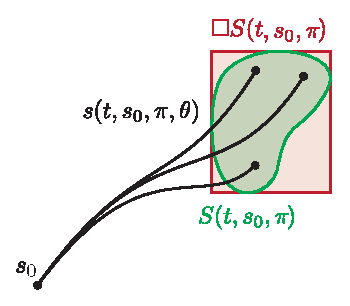
\includegraphics[width=0.3\textwidth]{img/interval-hull}
    \caption{A few trajectories are sampled from an initial state $x_0$ following a policy $\bu=(u_0,\cdots)$ with various parameters $\theta$ (in black). The union of reachability sets is shown in green, and its interval hull in red.}
    \label{fig:interval-hull}
\end{figure}

In order to use the interval predictor from \citep{leurent2019interval}, we need an additional assumption.

% \begin{lemma}[Similarity Transformation]
% \label{lem:metzler} Let $D\in\Xi\subset\Real^{n\times n}$ be a matrix variable satisfying the interval constraints $\Xi=\{D\in\Real^{n\times n}:\,D_{a}-\Delta\le D\le D_{a}+\Delta\}$ for some $D_{a}^{\text{T}}=D_{a}\in\Real^{n\times n}$ and $\Delta\in\Real_{+}^{n\times n}$. If for some constant $\mu\in\Real_{+}$ and a diagonal matrix $\Upsilon\in\Real^{n\times n}$ the Metzler matrix $Y=\mu E_{n\times n}-\Upsilon$ has the same eigenvalues as the matrix $D_{a}$, then there is an orthogonal matrix $S\in\Real^{n\times n}$ such that the matrices $S^{\text{T}}DS$ are Metzler for all $D\in\Xi$ provided that $\mu>n||\Delta||_{max}$.\textup{ }
% \end{lemma}

\begin{assumption}
There exists an orthogonal $S\in\Real^{d\times d}$ such that $S^\transp A_0 S$ is Metzler.
\end{assumption}

This for instance the case when $A_0$ is diagonalizable. Another way ... the similarity transformation of \citep{Efimov_a2013}.

\begin{theorem}[Interval Predictor \citep{leurent2019interval}]
\label{thm:predictor}
Assuming that \eqref{eq:polytope} is satisfied for the system \eqref{eq:dynamics}, then the interval predictor:
\begin{eqnarray}
\dot{\underline{x}}(t) & = & A_{0}\underline{x}(t)-\Delta A_{+}\underline{x}^{-}(t)-\Delta A_{-}\overline{x}^{+}(t)\nonumber \\
 &  & +Bu(t)+D^{+}\underline{\omega}(t)-D^{-}\overline{\omega}(t),\nonumber\\
\dot{\overline{x}}(t) & = & A_{0}\overline{x}(t)+\Delta A_{+}\overline{x}^{+}(t)+\Delta A_{-}\underline{x}^{-}(t) \label{eq:interval_predictor} \\
 &  & +Bu(t)+D^{+}\overline{\omega}(t)-D^{-}\underline{\omega}(t),\nonumber \\
 &  & \underline{x}(0)=\underline{x}_{0},\;\overline{x}(0)=\overline{x}_{0}\nonumber 
\end{eqnarray}
ensures the inclusion property \eqref{eq:interval_property}.

% Moreover, the stability of the predictor can be assessed with a sufficient condition in form of an LMI.
% if there exist diagonal matrices $P$, $Q$, $Q_{+}$, $Q_{-}$, $Z_{+}$, $Z_{-}$, $\Psi_{+}$, $\Psi_{-}$, $\Psi$, $\Gamma\in\Real^{2n\times 2n}$ such that the following LMIs are satisfied:
% \begin{gather*}
% P+\min\{Z_{+},Z_{-}\}>0,\;\Upsilon\preceq0,\;\Gamma>0,\\
% Q+\min\{Q_{+},Q_{-}\}+2\min\{\Psi_{+},\Psi_{-}\}>0,
% \end{gather*}
% where{\footnotesize{}
% \begin{gather*}
% \Upsilon=\left[\begin{array}{cccc}
% \Upsilon_{11} & \Upsilon_{12} & \Upsilon_{13} & P\\
% \Upsilon_{12}^{\top} & \Upsilon_{22} & \Upsilon_{23} & Z_{+}\\
% \Upsilon_{13}^{\top} & \Upsilon_{23}^{\top} & \Upsilon_{33} & Z_{-}\\
% P & Z_{+} & Z_{-} & -\Gamma
% \end{array}\right],\\
% \Upsilon_{11}=\mathcal{A}^{\top}P+P\mathcal{A}+Q,\;\Upsilon_{12}=\mathcal{A}^{\top}Z_{+}+PR_{+}+\Psi_{+},\\
% \Upsilon_{13}=\mathcal{A}^{\top}Z_{-}+PR_{-}+\Psi_{-},\;\Upsilon_{22}=Z_{+}R_{+}+R_{+}^{\top}Z_{+}+Q_{+},\\
% \Upsilon_{23}=Z_{+}R_{-}+R_{+}^{\top}Z_{-}+\Psi,\;\Upsilon_{33}=Z_{-}R_{-}+R_{-}^{\top}Z_{-}+Q_{-},\\
% \mathcal{A}=\left[\begin{array}{cc}
% A_{0} & 0\\
% 0 & A_{0}
% \end{array}\right],\;R_{+}=\left[\begin{array}{cc}
% 0 & -\Delta A_{-}\\
% 0 & \Delta A_{+}
% \end{array}\right],\;R_{-}=\left[\begin{array}{cc}
% \Delta A_{+} & 0\\
% -\Delta A_{-} & 0
% \end{array}\right],
% \end{gather*}
% }then the predictor \eqref{eq:interval_predictor} is input-to-state stable with respect to the inputs $\underline{\omega}$, $\overline{\omega}$.
\end{theorem}

We consider interval prediction rather than zonotope prediction for instance, for the sake of simplicity of implementation and computational efficiency. Among interval prediction algorithms, this predictor tends to produce tighter and more stable predictions than other candidates, and its stability can be assessed simply in terms of LMI.

% \begin{example*}
% Consider a scalar system:
% \[
% \dot{x}(t)=-\theta(t)x(t)+d(t),\;t\geq0,
% \]
% where $x(t)\in\Real$ with $x(0)\in[\underline{x}_{0},\overline{x}_{0}]=[1.0, 1.1]$, $\theta(t)\in\Pi=[\underline{\theta},\overline{\theta}]=[0.5,1.5]$ and $d(t)\in[\underline{d},\overline{d}]=[-0.1,0.1]$ for all $t\geq0$. The \autoref{fig:predictor_example} shows the state-interval obtained with \eqref{eq:interval_predictor}.

% \begin{figure}
% \begin{centering}
% 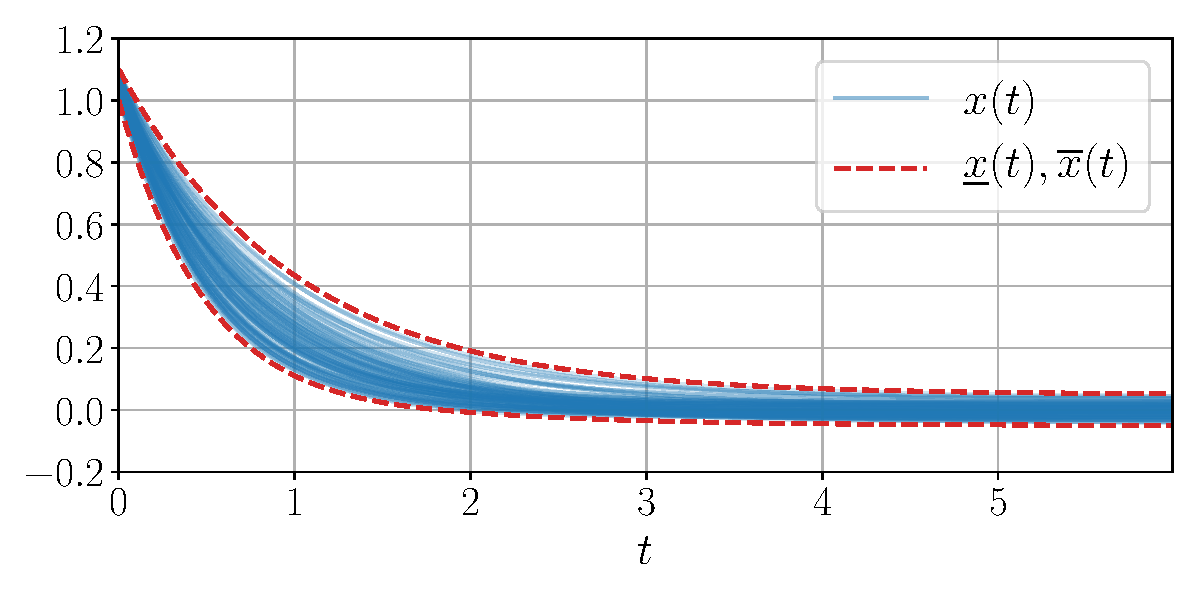
\includegraphics[width=\linewidth]{img/interval_predictor}
% \par\end{centering}
% \caption{Several trajectories for different values of $\theta\in\Theta$ are shown in blue. The result of prediction by \eqref{eq:interval_predictor} is in red: the predictor is stable and produces tight bounds.}
% \label{fig:predictor_example}
% \end{figure}
% \end{example*}

\section{Control}

At time $N$, we denote the vector of future controls as $\bu = (u_{N+1},u_{N+2},\cdots)$ and future perturbations as $\bw = (\omega_N, \omega_{N+1},\cdots)$.

We consider the robust control objective $V^r$:

\begin{equation}
\label{eq:robust-control}
\max_\bu \underbrace{\min_{\substack{A(\theta) \in \cP \\ \bw\in[\underline{\omega},\overline{\omega}]^\Natural}} \left[\sum_{t=0}^\infty \gamma^t r(x(t,\bu,\bw))\right]}_{V^r(\bu)}
\end{equation}


\begin{definition}[Surrogate objective]
We approximate the robust objective $V^r$ in \eqref{eq:robust-control} by replacing the true reachability set by its interval prediction $[\underline{x}(t), \overline{x}(t)]$ based on the dynamics confidence region $\cC_\delta$:

\begin{align}
\underline{R}(t,\bu) \eqdef \min_{x\in[\underline{x}(t, \bu), \overline{x}(t, \bu)]}  R(x) \\
\hat{V}^r(\bu) \eqdef \sum_{t=0}^\infty \gamma^t \underline{R}(t,\bu) \label{eq:surrogate_objective}
\end{align}
where $\underline{x}(t, \bu), \overline{x}(t, \bu)$ follow the dynamics defined in \eqref{eq:interval_predictor}.
\end{definition}

This does not amount to defining a pessimistic reward-function $\underline{R}$, since the worst case is assessed over the whole trajectory being optimized, and not at the level of a local transition. It cannot be precomputed prior to the control optimization procedure, it needs to be done jointly.

%\begin{algorithm}[tp]
%  \SetAlgoLined\DontPrintSemicolon
%  \SetKwFunction{algo}{robust\_control}
%  \SetKwFunction{proc}{pessimistic\_step}
%  \SetKwProg{myalg}{Algorithm}{}{}
%  \myalg{\algo{$s_0$}}{
%  \While{resources available}
%  {
%  Select a candidate action sequence $a$ with a planning algorithm.\;
%  Sample a pessimistic transition and reward $\underline{r}_t$ using \proc{$\underline{x}(t)$, $\overline{x}(t)$, a}.
% \;
% Update the planning algorithm with the sampled pessimistic transition.
%  }
%  \KwRet $\argmax_{\bu} \hat{v^r}(\bu)$ \;}{}
%  \setcounter{AlgoLine}{0}
%  \SetKwProg{myproc}{Procedure}{}{}
%  \myproc{\proc{$\underline{x}(t)$, $\overline{x}(t)$, $a$}}{
%  Integrate \eqref{eq:interval_predictor} over $dt$ with controls $a$ to compute $\underline{x}(t+dt), \overline{x}(t+dt)$\;
%  Compute worst-case reward $\underline{r}_t = \min_{x\in[\underline{x}(t), \overline{x}(t)]} r(x)$\;
%  \KwRet $\underline{x}(t+dt), \overline{x}(t+dt), \underline{r}_t$\;}
%\caption{Interval-based Robust Control}
%\label{algo:irc}
%
%\end{algorithm}

\begin{proposition}[Lower bound]
\label{prop:lower-bound}
With high probability, the surrogate objective $\hat{V}^r$ is a lower bound of the true objective $V^r$:

\begin{equation}
\hat{V}^r(\bu) \leq V^r(\bu)
\end{equation}
\end{proposition}

Since all our approximations were conservative, if we manage to find a control sequence such that no \textit{bad event} (e.g. a collision) happens with our surrogate objective, then we are guaranteed so they will not happen either when the controls are executed on the true system.

\begin{proposition}
\label{prop:control-error}
If we assume that the reward function $R$ is lipschitz, then we can bound the approximation error:
\begin{equation*}
     V^r(\bu) - \hat{V}^r(\bu) = \cO\left(\frac{1}{\sqrt{N}}\right)
\end{equation*}
\end{proposition}

\begin{algorithm}[tb]
   \caption{Robust Estimation, Prediction and Control}
   \label{alg:full}
\begin{algorithmic}
   \STATE {\bfseries Input:} confidence level $\delta$
   \FOR{$N = 1,2,3,\dots$} 
   \STATE Compute the dynamics confidence region $\cC_{[N],\delta}$ with \textsc{Model Estimation} \eqref{eq:generic-polytope} on $\cD_{[N]}$.
   \FOR{planning steps $[T]$}
   \STATE Get the tree node $\bu^t$ to expand with \textsc{Pessimistic Planning}  \eqref{eq:surrogate_objective} using $[\underline{x}(t,\bu), \overline{x}(t,\bu)]$.
   \STATE For each child transition, simulate $[\underline{x}, \overline{x}]$ with \textsc{Interval Prediction} \eqref{eq:interval_predictor} using $\cC_{[N],\delta}$.
   \ENDFOR
   \STATE Execute the first recommended control $u_N$, and add the observed transition $(x_N, u_N, \dot{x}_N)$ to $\cD_{[N+1]}$.
   \ENDFOR
   
\end{algorithmic}
\end{algorithm}

\section{Multi-model Extension}

The procedure we developed in sections relies on several modelling assumptions which can be quite restrictive, such as the system dynamics \eqref{eq:dynamics} or its linear parametrisation in \autoref{assumpt:linear_param}. But what if they are wrong?

\paragraph{Model adequacy}

We can test the model adequacy, and eventually reject it.

This suggest using multiple models with different sets of features.

\subsection{Robust control with Discrete Ambiguity}


\begin{assumption}[Multi-model ambiguity]
Assume that the true dynamics $f$ lies within a finite set of candidate models $f^1, \cdots, f^M$.
\begin{equation}
\exists m\in[M]: \dot{x}(t) = f^M(x(t), u(t)), \forall t\geq 0
\end{equation}

We temporarily ignore the parametric uncertainty $\theta\in\Theta$ to only consider known deterministic models.
\end{assumption}

\begin{definition}[Robust sequence upper bounds] We define an upper-bound for the value of sequences of actions:
\begin{equation}
\label{eq:robust_sequence_ucb}
b_i^r(n)  \eqdef
\begin{cases}
\min_{m\in[1, M]} \sum_{t=0}^{d-1} \gamma^t R_t^m  + \frac{\gamma^d}{1-\gamma} &\text{if } i \in \mathcal{L}_n \text{ ;}\\
\max_{a\in\mathcal{A}} B_{ia}^r(n) & \text{if } i \in \mathcal{T}_n \setminus \mathcal{L}_n 
\end{cases}
\end{equation}
where $R_t^m$ is the reward obtained at step $t$ by following $i$ with dynamics $f^m$.
\end{definition}
An illustration of the computation of the robust b-values is presented in Figure \ref{fig:drop}.

\begin{figure}
\centering
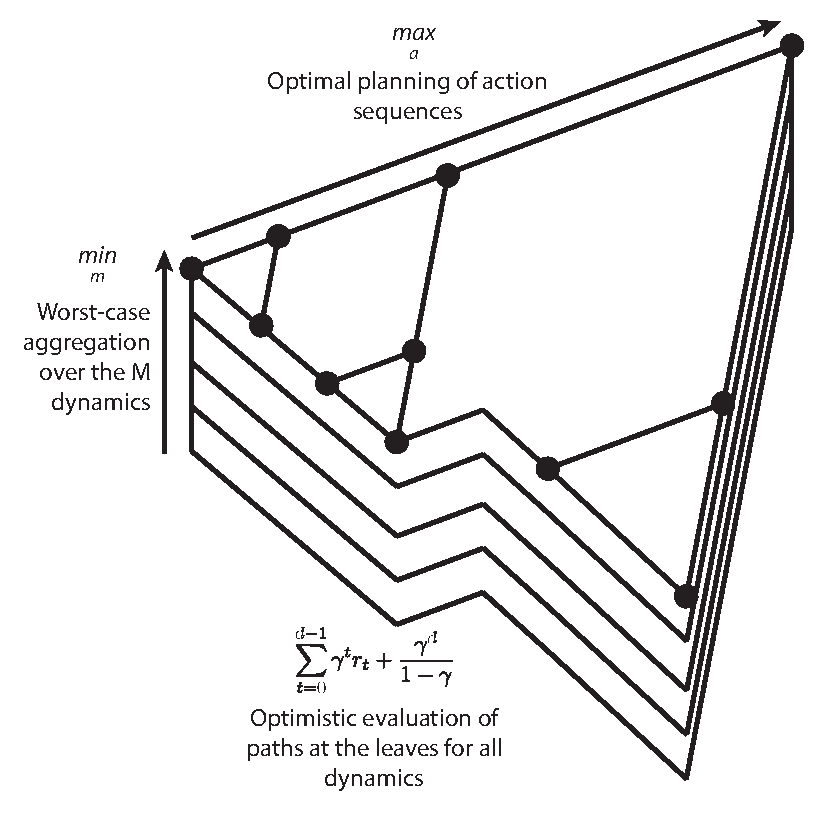
\includegraphics[width=0.4\linewidth]{img/robust-control-tree}
\caption{The computation of robust B-values in Algorithm \ref{algo:drop}. The simulation of trajectories for every dynamics model $f^m$ is represented as stacked versions of the expanded tree $\mathcal{T}_n$.}
\label{fig:drop}
\end{figure}

From this definition we introduce Algorithm \ref{algo:drop}, and analyse its sample-efficiency in Theorem \ref{theorem:drop-regret}.

%\begin{algorithm}[tp]
%\DontPrintSemicolon
%Initialize $\mathcal{T}$ to a root and expand it. Set $n=1$.\;
%\While{Numerical resource available for episode $n$}{
%Compute the robust b-values $b^r_i(n)$.\;
%Expand the leaf $\argmax_{i\in \mathcal{L}_n} b^r_i(n)$.\;
%}
%\Return $\argmax_{a\in \mathcal{A}} u^r_a(n)$
%\caption{Deterministic Robust Optimistic Planning}
%\label{algo:drop}
%\end{algorithm}

We express the performance of the planning problem in terms of a measure of the proportion of near-optimal paths:
\[
\kappa = \limsup_{h\rightarrow\infty} \left|\left\{a\in A^h: V(a)\geq V - \frac{\gamma^{h+1}}{1-\gamma}\right\}\right|^{1/h}.
\]

\begin{theorem}[Regret bound]
\label{theorem:drop-regret}
The simple regret of Algorithm \ref{algo:drop} after $T$ iterations is:

\begin{equation}
\text{If } \kappa>1,\qquad 
v^r - v^r_{a_T} = O\left(T^{-\frac{\log 1/\gamma}{\log \kappa}}\right)
\end{equation}

\begin{equation}
\text{If }\kappa=1,\qquad
v^r - v^r_{a_T} = O\left(\gamma^{\frac{(1-\gamma)^\beta}{c}T}\right)
\end{equation}
\end{theorem}

\section{Experiments}

We consider the problem of safe decision-making for an autonomous vehicle. An autonomous vehicle is driving on a highway populated with $N$ other agents, and uses Model Predictive Control to plan a sequence of decisions. To that end, it relies on parametrized dynamical model for each agent to predict the future trajectory of each traffic participant: \[\dot{z}_i=f_i(Z,\theta_i),\;i=\overline{1,N},\] where $f_i$ are described below, $z_i\in\Real^4$ is the state of an agent, $Z = [z_1,\dots,z_N]^\top\in\Real^{4N}$ and $\theta_i\in\Real^5$ is the corresponding vector of unknown parameters. Crucially, this system describes the couplings and interactions between vehicles, so that the autonomous agent can properly anticipate their reactions. 
However, we assume that we do not have access to the true values of the behavioural parameters $\theta=[\theta_1,\dots,\theta_N]^\top$; instead, we merely know that these parameters lie in a set of admissible values $\Theta\subset\Real^{5N}$. In order to act safely in the face of uncertainty, we follow the framework of robust decision-making: the agent must consider all the possible trajectories in the space of $Z$ that each vehicle can follow in order to take its decisions. In this work, we focus on how to compute these trajectory enclosures through interval prediction.

The system 


\bibliography{references}
\bibliographystyle{icml2020}

\clearpage
\appendix

\section{Proofs}

\subsection{Proof of \autoref{prop:regularized_solution}}

\begin{proof}
We differentiate $J(\theta) = \sum_{n=1}^N \|y_n -\Phi_n\theta\|_{\Sigma_p^{-1}}^2 + \lambda\|\theta\|_{}^2$ as in  \eqref{eq:regression_min} with respect to $\theta$:

\begin{align*}
    \nabla_{\theta} J(\theta) &= \sum_{n=1}^N\nabla_{\theta} (y_n - \Phi_n\theta)^\transp\Sigma_p^{-1}(y_n - \Phi_n\theta) + \nabla_{\theta} \lambda\|\theta\|_{}^2\\
    &= -2\sum_{n=1}^N y_n^\transp\Sigma_p^{-1}\Phi_n + 2\sum_{n=1}^N\theta^\transp(\Phi_n^\transp\Sigma^{-1}\Phi_n) +  2 \lambda \theta^\transp
\end{align*}

Hence,
\begin{align*}
    \nabla_{\theta} J(\theta) = 0 \iff \left(\sum_{n=1}^N\Phi_n^\transp\Sigma_p^{-1}\Phi_n + I_d\right)\theta = \sum_{n=1}^N y_n^\transp\Sigma_p^{-1}\Phi_n
\end{align*}
\end{proof}

\subsection{Proof of \autoref{prop:concentration}}

\begin{proof}


Let 
\begin{equation*}
    G_t = \sum_{s=1}^t \Phi_s^\transp \Sigma_p^{-1} \Phi_s \in \Real^{d\times d}
\end{equation*}
And for any $z\in\Real^d$,
\begin{equation*}
    M_t^z = \exp{\left(\inp{z}{S_t} - \frac{1}{2}\|z\|_{G_t}\right)}
\end{equation*}
\begin{equation*}
    D_t^z = \exp{\left(\inp{\Phi_t z}{\eta_t}_{\Sigma_p^{-1}} - \frac{1}{2}\|\Phi_t z\|_{\Sigma_p^{-1}}\right)}
\end{equation*}
Then,
\begin{align*}
    M_t^z = \exp{\left(\sum_{s=1}^t z^\transp \Phi_s^\transp \Sigma_p^{-1} \eta_s - \frac{1}{2} (\Phi_s z)^\transp\Sigma_p^{-1}(\Phi_s z) \right)} = \prod_{s=1}^{t} D_s^z
\end{align*}
and using the Sub-Gaussianity of $\eta_t$
\begin{align*}
    \expectedvalue\left[D_t^z \condbar F_{t-1}\right] = {}& \exp{\left(- \frac{1}{2}\|\Phi_t z\|_{\Sigma_p^{-1}}\right)}\\ &\expectedvalue\left[\exp{\left(\inp{\Phi_t z}{\eta_t}_{\Sigma_p^{-1}}\right)} \condbar F_{t-1}\right]  \\
    \leq {} & \exp{\left(- \frac{1}{2}\|\Phi_t z\|_{\Sigma_p^{-1}}\right)}\\
    &\exp{\left((z^\transp \Phi_t^\transp \Sigma_p^{-1})\Sigma_p(\Sigma_p^{-1} \Phi_t z)\right)}\\
    &= 1
\end{align*}
\begin{align*}
    \expectedvalue\left[M_t^z \condbar F_{t-1}\right] = \left(\prod_{s=1}^{t-1} D_s^z\right) \expectedvalue\left[D_t^z \condbar F_{t-1}\right] \leq M_{t-1}^z
\end{align*}
Showing that $(M_t^z)_{t=1}^\infty$ is indeed a supermartingale and in fact $\expectedvalue[M_t^z]\leq 1$.
I then follows by Doob's upcrossing lemma for super-martnigales that $M_\infty^z = \lim_{t\to\infty} M_t^z$ is almost surely well-defined, ans so is $M_\tau^z$ for any random stopping time $\tau$.

Next, we consider the stopped martingale $M_{\min(\tau,t)}^z$. Since 
$(M_t^z)_{t=1}^\infty$ is a non-negative supermartingale and $\tau$ is a random stopping time, we deduce by Doob's decomposition that
\begin{align*}
\expectedvalue[M_{\min(\tau,t)}^z] &= \expectedvalue[M_0^z] + \expectedvalue[\sum_{s=0}^{t-1} (M_{s+1}^z-M_s^z) \mathbb{I}\{\tau>s\}]\\
&\leq 1 + \expectedvalue[\sum_{s=0}^{t-1} \expectedvalue[M_{s+1}^z-M_s^z|F_{s}] \mathbb{I}\{\tau>s\}]\\
&\leq 1
\end{align*}
Finally, an application of Fatou's lemma show that 
$\expectedvalue[M_\tau^z] = \expectedvalue[\liminf_{t\to\infty} M_{\min(\tau,t)}^z] \leq \liminf_{t\to\infty} \expectedvalue[M_{\min(\tau,t)}^z] \leq 1.$

% The following uses the method of mixtures.
% Let $\Gamma$ be a Gaussian random variable which is independent of all other random variables and whose covariance is $\Sigma^{-1}$. (in our estimator, $\Sigma = \lambda$).

% Define 
% \[
% M_t = \expectedvalue \left[M_t^\Gamma \condbar F_\infty\right]
% \]

% where $F_\infty$ is the tail $\sigma$-algebra of the filtration. Clearly, we still have $\expectedvalue[M_\tau] = \expectedvalue[\expectedvalue[M_\tau^\Gamma|\Gamma]]\leq 1$.

% Let us calculate $M_t$. Let $f$ denote the density of $\Gamma$ and for a positive definite matrix $P$ let $c(P) = \sqrt{(2\pi)^d/\det(P)} = \int \exp (-\frac{1}{2}x^\transp P x)$


\begin{lemma}[Theorem 14.7 of \citep{pena2008self}]
If $Z$ is a random vector and $B$ is a symmetric positive definite matrix such that
\[\forall \gamma\in\Real^d, \ln \expectedvalue \exp \left(\gamma^\transp Z -\frac{1}{2} \gamma^\transp B \gamma \right)\leq 0,\]
then for any positive definite non-random matrix C, it holds
\[\expectedvalue\left[ \sqrt{\frac{\det(C)}{\det(B+C)} } \exp\left( \frac{1}{2}\|Z\|^2_{(B+C)^{-1}}\right)\right]\leq 1. \] 
In particular, by Markov inequality, for all $\delta\in(0,1)$, 
\[\probability{\|Z\|_{(B+C)^{-1}} \geq \sqrt{2\ln \left(\frac{\det \left((B+C)^{1/2}\right)}{\delta\det(C)^{1/2}}\right)}}\leq \delta.\]
\end{lemma}

Here, by using $Z = \sum_{s=1}^t\Phi_s\Sigma_p^{-1}\eta_s$, $B=G_t$, $C=G$,

\[
\probability{\| S_t \|_{(G_t+G)^{-1}} \geq \sqrt{2\ln \left(\frac{\det(G_t+G)^{1/2}}{\delta\det(G)^{1/2}}\right)}} \leq \delta
\]

\end{proof}

\subsection{Proof of \autoref{thm:confidence_ellipsoid}}

\begin{proof}

Hence, for all $x\in\Real^d$,
\begin{align*}
    x^\transp\theta_{N,\lambda}  -x^\transp\theta &= x^\transp G_{N, \lambda}^{-1}\sum_{n=1}^N \Phi_n^\transp \Sigma_p^{-1}\eta_n
    - \lambda x^\transp G_{N, \lambda}^{-1}\theta\\
    &= \inp{x}{\sum_{n=1}^N \Phi_n^\transp \Sigma_p^{-1}\eta_n}_{G_{N, \lambda}^{-1}} - \lambda\inp{x}{\theta}_{G_{N, \lambda}^{-1}}
\end{align*}

Using the Cauchy-Schwartz inequality, we get:
\begin{align*}
    |x^\transp\theta_{N,\lambda}  -x^\transp\theta| &\leq \|x\|_{G_{N, \lambda}^{-1}}\left(\left\|\sum_{n=1}^N \Phi_n^\transp \Sigma_p^{-1}\eta_n\right\|_{G_{N, \lambda}^{-1}} + \lambda\|\theta\|_{G_{N, \lambda}^{-1}}\right)
\end{align*}

In particular, for $x = G_{N,\lambda}(\theta_{N,\lambda} - \theta)$, we get after simplifying with $\| \theta_{N,\lambda}  - \theta\|_{G_{N,\lambda}}$:
\begin{align*}
    \| \theta_{N,\lambda}  - \theta\|_{G_{N,\lambda}} &\leq \left\|\sum_{n=1}^N \Phi_n^\transp \Sigma_p^{-1}\eta_n\right\|_{G_{N, \lambda}^{-1}} + \lambda\|\theta\|_{G_{N, \lambda}^{-1}}
\end{align*}

By applying \autoref{prop:concentration} with $G=\lambda I_d$, we obtain that with probability at least $1-\delta$,
\begin{align*}
    \| \theta_{N,\lambda}  - \theta\|_{G_{N,\lambda}} &\leq \sqrt{2\ln \left(\frac{\det(G_{N,\lambda})^{1/2}}{\delta\det(\lambda I_d)^{1/2}}\right)}
     + \lambda\|\theta\|_{G_{N, \lambda}^{-1}}
\end{align*}
And since $\|\theta\|_{G_{N, \lambda}^{-1}}^2 \leq 1/\lambda_{\min}(G_{N,\lambda})\|\theta\|_2^2 \leq 1/\lambda \|\theta\|_2^2$,
\begin{align*}
    \| \theta_{N,\lambda}  - \theta\|_{G_{N,\lambda}} &\leq \sqrt{2\ln \left(\frac{\det(G_{N,\lambda})^{1/2}}{\delta\det(\lambda I_d)^{1/2}}\right)}
     + \lambda^{1/2}\|\theta\|_2
\end{align*}
\end{proof}


\subsection{Proof of \autoref{prop:lower-bound}}

\begin{proof}
We have that $A(\theta) \in \cC_{[N],\delta}$ with probability $1-\delta$. Whenever it is the case, we have by \autoref{thm:predictor} that the inclusion property \eqref{eq:interval_property} is verified by the interval predictor \eqref{eq:interval_predictor} for all $\omega(t)\in[\underline{\omega}(t), \overline{\omega}(t)]$. This gives the following bound:
\begin{equation*}
 \sum_{t=0}^\infty \gamma^t r(x_t) \geq \sum_{t=0}^\infty \min_{x\in[\underline{x}(t, \bu), \overline{x}(t, \bu)]} \gamma^t r(x) = \hat{v^r}(\bu)
\end{equation*}

And finally, with probability $1-\delta$,
\begin{align*}
v^r(\bu) &= \min_{A(\theta) \in A(\Theta)} \expectedvalueover{\omega(t)}\left[\sum_{t=0}^\infty \gamma^t r(x_t)\right] \\
&\geq \min_{A \in \cP} \expectedvalueover{\omega(t)}\left[\sum_{t=0}^\infty \gamma^t r(x_t)\right] \\
& \geq \min_{A \in \cP} \expectedvalueover{\omega(t)}\left[\hat{v^r}(\bu)\right] = \hat{v^r}(\bu)
\end{align*}
\end{proof}

\section{The use case of autonomous driving}

In the following, we describe the structure of the model representing the dynamics of of several vehicles driving and interacting with one another.

\subsection{Kinematics}

The kinematics of any vehicle $i\in\overline{1,V}$ are represented by the Kinematic Bicycle Model:
\begin{align}
	\dot{x}_i &= v_i\cos(\psi_i), \nonumber\\
	\dot{y}_i &= v_i\sin(\psi_i), \nonumber\\
	\dot{v}_i &= a_i, \nonumber\\
	\dot{\psi}_i &= \frac{v_i}{l}tan(\beta_i), \nonumber
\end{align}
where $(x_i, y_i)$ is the vehicle position, $v_i$ is its forward velocity and $\psi_i$ is its heading, $l$ is the vehicle half-length, $a_i$ is the acceleration command and $\beta_i$ is the slip angle at the centre of gravity, used as a steering command.

\subsection{Longitudinal control}
Longitudinal behaviour is modelled by a linear controller using three features inspired from the intelligent driver model (IDM) \cite{Treiber2000}: a desired velocity, a braking term to drive slower than the front vehicle, and a braking term to respect a safe distance to the front vehicle.

Denoting $f_i$ the index of the front vehicle preceding vehicle $i$, the acceleration command can be presented as follows:
\begin{equation*}
	a_i = \begin{bmatrix}
	\theta_{i,1} & \theta_{i,2} & \theta_{i,3}
	\end{bmatrix} \begin{bmatrix}
		v_0 - v_i \\
		-(v_{f_i}-v_i)^- \\
		-(x_{f_i} - x_i - (d_0 + v_iT))^- \\
	\end{bmatrix},
	\label{eq:theta_a}
\end{equation*}
where $v_0, d_0$ and $T$ respectively denote the speed limit, jam distance and time gap given by traffic rules.

\subsection{Lateral control}

The lane $L_i$ with the lateral position $y_{L_i}$ and heading $\psi_{L_i}$ is tracked by a cascade controller of lateral position and heading $\beta_i$, which is selected in a way the closed-loop dynamics take the form:

\begin{align}
	\label{eq:heading-command}
    \dot{\psi}_i &= \theta_{i,5}\left(\psi_{L_i}+\sin^{-1}\left(\frac{\tilde{v}_{i,y}}{v_i}\right)-\psi_i\right),\\
    \tilde{v}_{i,y} &= \theta_{i,4} (y_{L_i}-y_i). \nonumber
\end{align}
We assume that the drivers choose their steering command $\beta_i$ such that \eqref{eq:heading-command} is always achieved: $\beta_i = \tan^{-1}(\frac{l}{v_i}\dot{\psi}_i)$.

\subsection{LPV formulation}

The system presented so far is non-linear and must be cast into the LPV form. We approximate the non-linearities induced by the trigonometric operators through equilibrium linearisation around $y_i=y_{L_i}$ and $\psi_i=\psi_{L_i}$.

This yields the following longitudinal dynamics:
\begin{align*}
\dot{x}_i &= v_i,\\
\dot v_i &= \theta_{i,1} (v_0 - v_i) + \theta_{i,2} (v_{f_i} - v_i) + \theta_{i,3}(x_{f_i} - x_i - d_0 - v_i T),
\end{align*}
where $\theta_{i,2}$ and $\theta_{i,3}$ are set to $0$ whenever the corresponding features are not active.

It can be rewritten in the form $$\dot{Z} = A(\theta)(Z-Z_c) + d.$$ For example, in the case of two vehicles only:
\begin{equation*}
    Z = \begin{bmatrix}
x_i \\
x_{f_i} \\
v_i \\
v_{f_i} \\
\end{bmatrix}
,\quad
Z_c = \begin{bmatrix}
-d_0-v_0 T \\
0 \\
v_0\\
v_0 \\
\end{bmatrix}
,\quad
d = \begin{bmatrix}
v_0 \\
v_0 \\
0\\
0\\
\end{bmatrix}
\end{equation*}

\begin{equation*}
A(\theta)
=
\begin{blockarray}{ccccc}
 & i & f_i & i & f_i \\
\begin{block}{c[cccc]}
i & 0 & 0 & 1 & 0 \\
f_i & 0 & 0 & 0 & 1 \\
i & -\theta_{i,3} & \theta_{i,3} & -\theta_{i,1}-\theta_{i,2}-\theta_{i,3} & \theta_{i,2} \\
f_i & 0 & 0 & 0 & -\theta_{f_i,1} \\
\end{block}
\end{blockarray}
\end{equation*}

The lateral dynamics are in a similar form:
\begin{equation*}
\begin{bmatrix}
\dot{y}_i \\
\dot{\psi}_i \\
\end{bmatrix}
=
\begin{bmatrix}
0 & v_i \\
-\frac{\theta_{i,4} \theta_{i,5}}{v_i} & -\theta_{i,5}
\end{bmatrix}
\begin{bmatrix}
y_i - y_{L_i} \\
\psi_i - \psi_{L_i}
\end{bmatrix}
+
\begin{bmatrix}
v_i\psi_{L_i} \\
0
\end{bmatrix}
\end{equation*}
Here, the dependency in $v_i$ is seen as an uncertain parametric dependency, \emph{i.e.} $\theta_{i,6}=v_i$, with constant bounds assumed for $v_i$ using an overset of the longitudinal interval predictor.

\subsection{Tighter conversion form ellipsoid to polytope}
\label{sec:tight-polytope}
\begin{lemma}[Confidence polytope]
\label{lem:tight_polytope}
We can enclose the confidence ellipsoid obtained in $\eqref{eq:confidence-ellipsoid}$ within a polytope $C_\delta$:
\begin{equation}
     \cC_\delta = \left\{ A_{1}+\sum_{i=1}^{2^d}\lambda_{i}\Delta A_{i}: \lambda\in[0, 1]^{2^d},  \sum_{i=1}^{2^d}\lambda_{i}=1\right\}.
\end{equation}
with 
\begin{align*}
    &h_k \text{ is the }k^\text{th}\text{ element of }\{-1,1\}^d\text{ for } k\in[2^d],\\
    &G_{N,\lambda}^{-1} = PDP^{-1}, \quad \Delta\theta_k = C_{N,\lambda,\delta}^{1/2} P^{-1}D^{-1/2} h_k, \\
    &A_0 = A + \theta_{N,\lambda}^\transp\Phi, \quad \Delta A_k = \Delta\theta_k^\transp\Phi.
\end{align*}
This conversion is illustrated in \autoref{fig:ellipsoid_to_polytope}.
\end{lemma}

\begin{proof}
The ellipsoid in \eqref{eq:confidence-ellipsoid} is described by:
\begin{align*}
    \theta\in\cC_\delta &\implies
    (\theta-\theta_{N,\lambda})^\transp G_{N,\lambda}^{-1}(\theta-\theta_{N,\lambda}) \leq C_{N,\lambda,\delta}\\
    &\implies (\theta'-\theta'_{N,\lambda})^\transp D (\theta'-\theta'_{N,\lambda}) \leq C_{N,\lambda,\delta}\\
    &\implies \sum_{i=1}^d D_{i,i}(\theta'_i-\theta'_{N,\lambda,i})^2\leq C_{N,\lambda,\delta}\\
    &\implies\forall i, |\theta'_i-\theta'_{N,\lambda,i}|\leq C_{N,\lambda,\delta}^{1/2}D_{i,i}^{-1/2}
\end{align*}
This describes a $\Real^d$ box containing $\theta' = P\theta$, whose $k^\text{th}$ vertex is represented by $\theta_{N,\lambda}' + C_{N,\lambda,\delta}^{1/2}D^{-1/2} h_k$. We obtain the corresponding box on $\theta$ by transforming each vertex of the box with $P^{-1}$.
\end{proof}

\begin{figure}
    \centering
    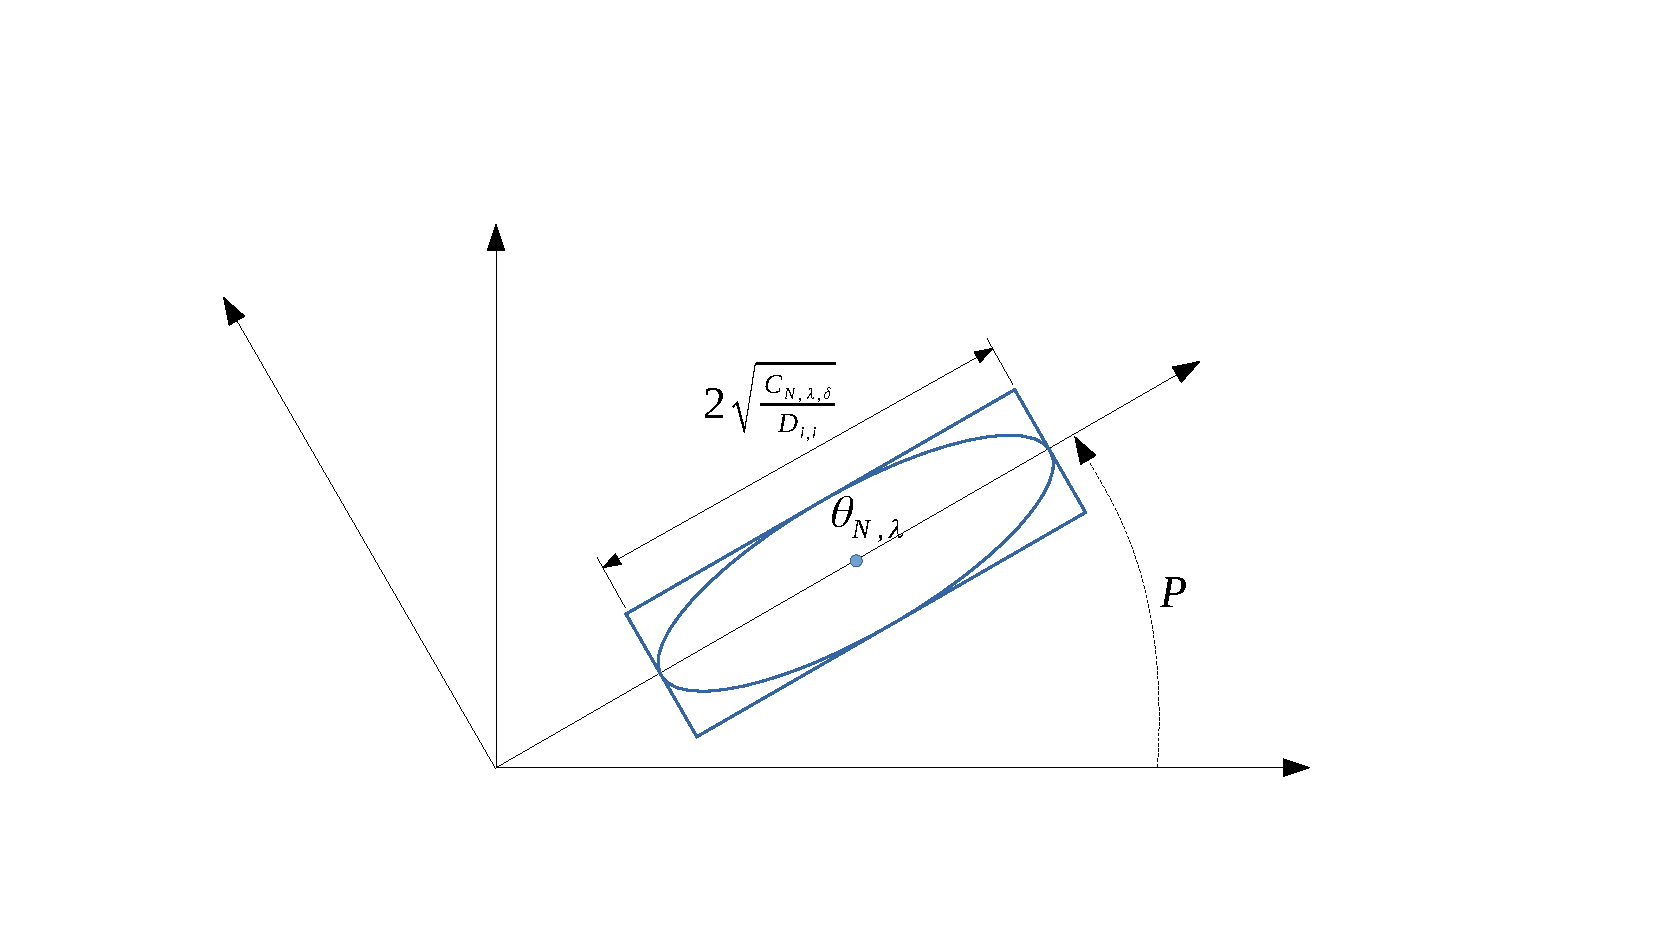
\includegraphics[trim={3.8cm, 2cm, 5cm, 3.8cm}, clip, width=0.4\textwidth]{img/ellipsoid_to_polytope}
    \caption{From the confidence ellipsoid $\cC_\delta$ to its enclosing polytope $\cP_\delta$}
    \label{fig:ellipsoid_to_polytope}
\end{figure}

\subsection{Change of coordinates}
In both cases, the obtained polytope centre $A_0$ is non-Metzler.
We use lemma \ref{lem:metzler} to compute a similarity transformation of coordinates. Precisely, we ensure that the polytope is chosen so that its centre $A_0$ is diagonalisable having real eigenvalues, and perform an eigendecomposition to compute its change of basis matrix $S$. The transformed system $Z'=S^{-1}(Z-Z_c)$ verifies \eqref{eq:polytope} with $A_0$ Metlzer as required to apply the interval predictor of Theorem~\ref{thm:predictor}. Finally, the obtained predictor is transformed back to the original coordinates $Z$ by using the interval arithmetic of Lemma~\ref{lem:interval}.


\end{document}
